\newpage
\section{КОНСТРУКТОРСКАЯ ЧАСТЬ}

\subsection{Разработка алгоритмов}

На вход у всех алгоритмов передаются в качестве параметров:
\begin{enumerate}
\item Адреса строк
\item Длины строк (не должны быть равна 0)
\item Адрес переменной, в которой будет храниться результат
\item Область памяти (для стандартных реализаций поиска редакционного расстояния), в которой сохраняется матрица с редакционными расстояниями
\end{enumerate}
Возвращаемое значение: код ошибки (0 в случае успеха, иначе отрицательное значение). \\
Побочные эффекты: изменяются значения в матрице и результата.

\newpage
\subsection{Схемы алгоритмов}

%Добавить сюда картинки из yEd
\begin{figure}[h!]
\center{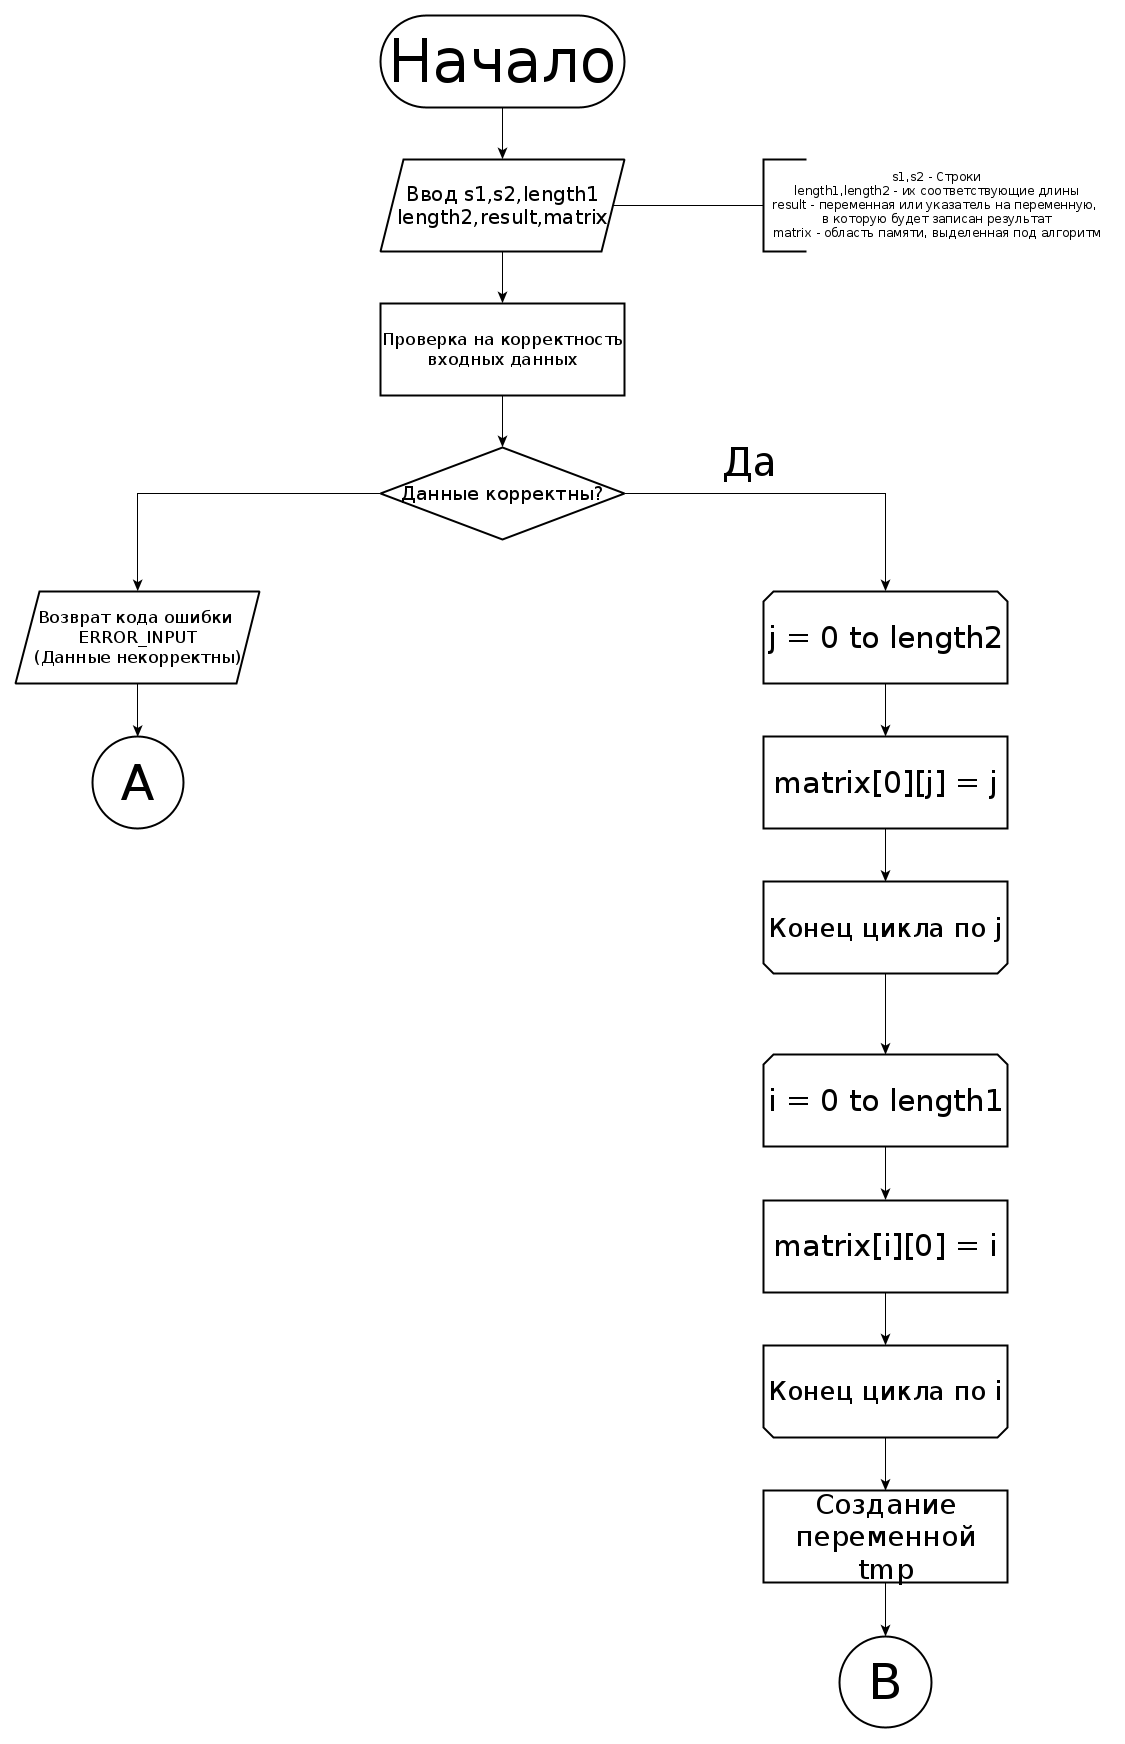
\includegraphics[scale=0.25]{levenstein.png}}
\caption{Схема стандартного алгоритма Левенштейна (Начало)}
\label{images:levenstein}
\end{figure}

\begin{figure}[p]
\center{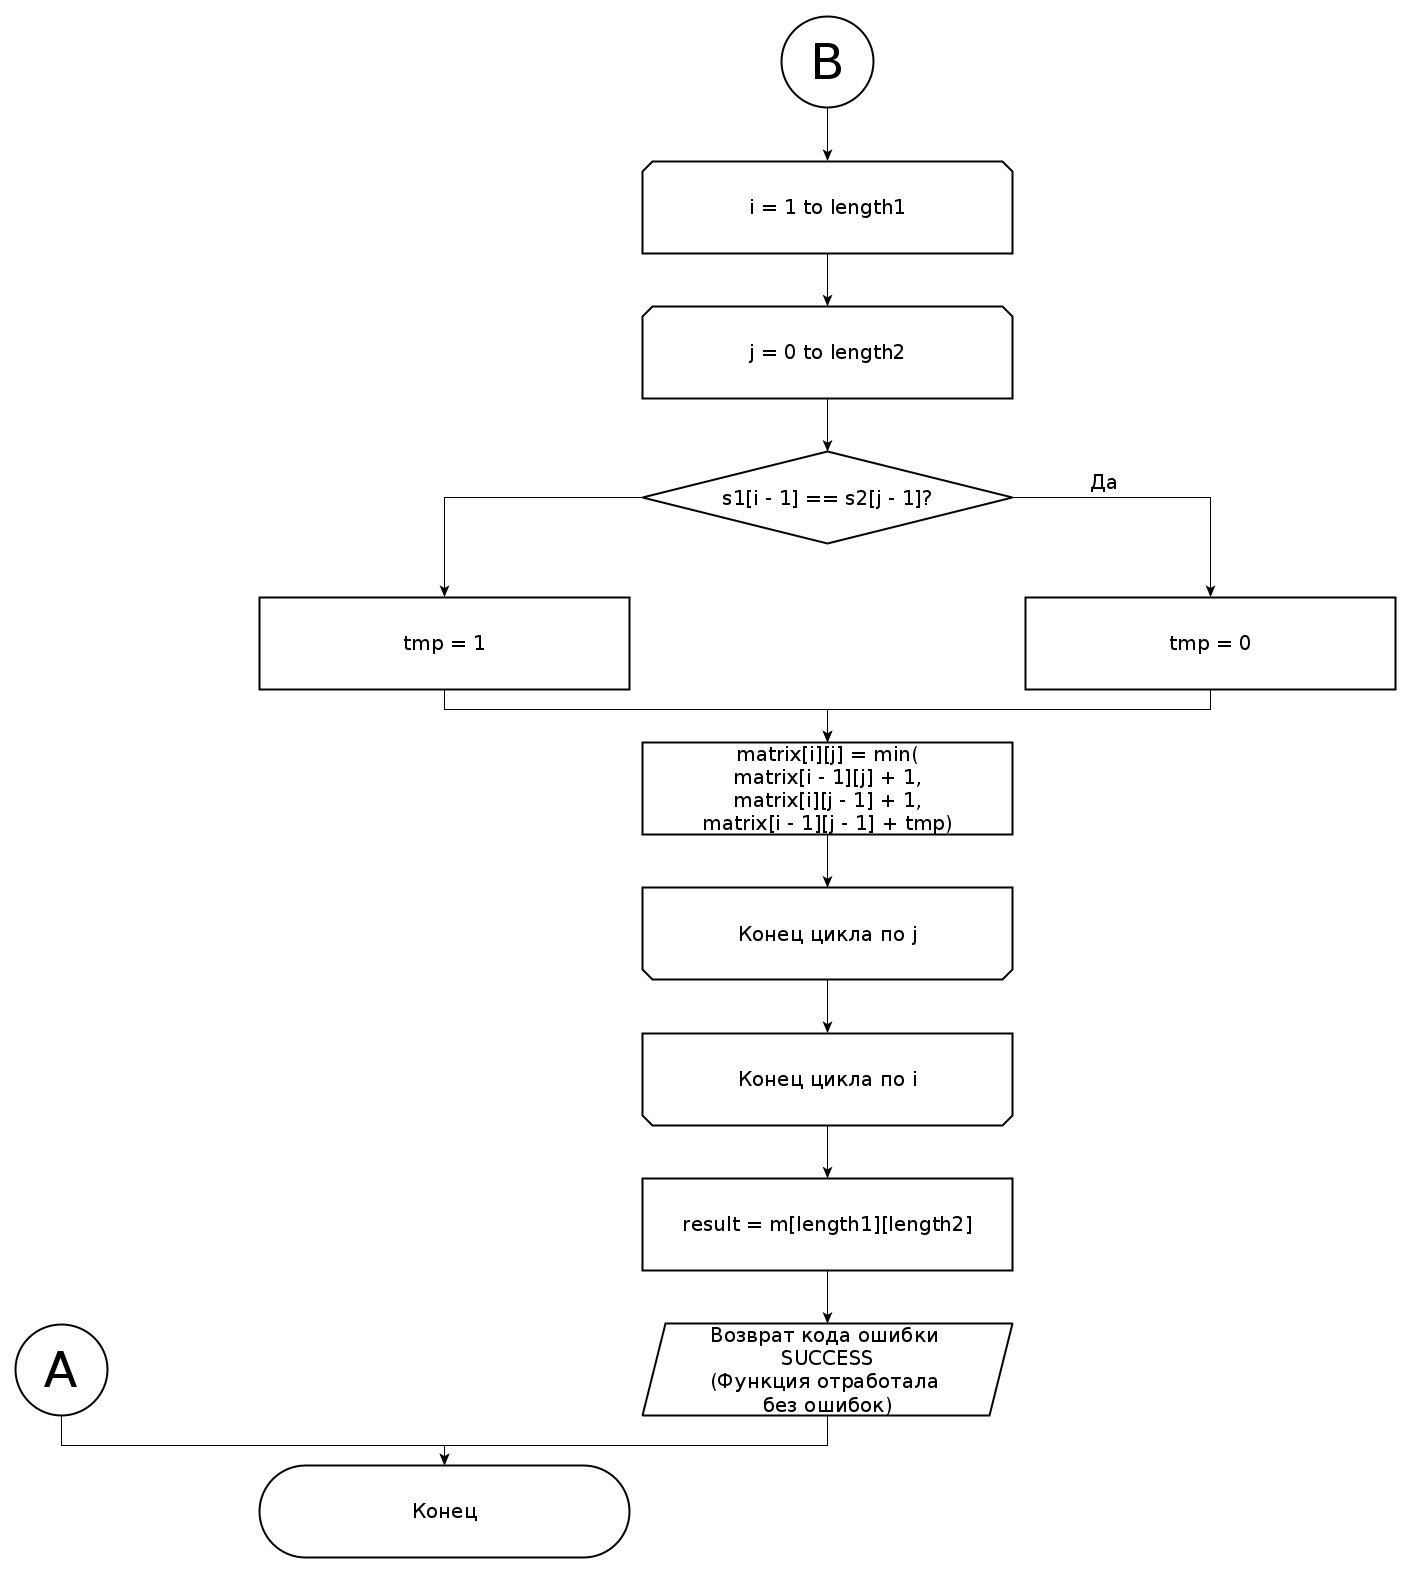
\includegraphics[scale=0.25]{levenstein2.png}}
\caption{Схема стандартного алгоритма Левенштейна (Конец)}
\label{images:levenstein2}
\end{figure}

\begin{figure}[p]
\center{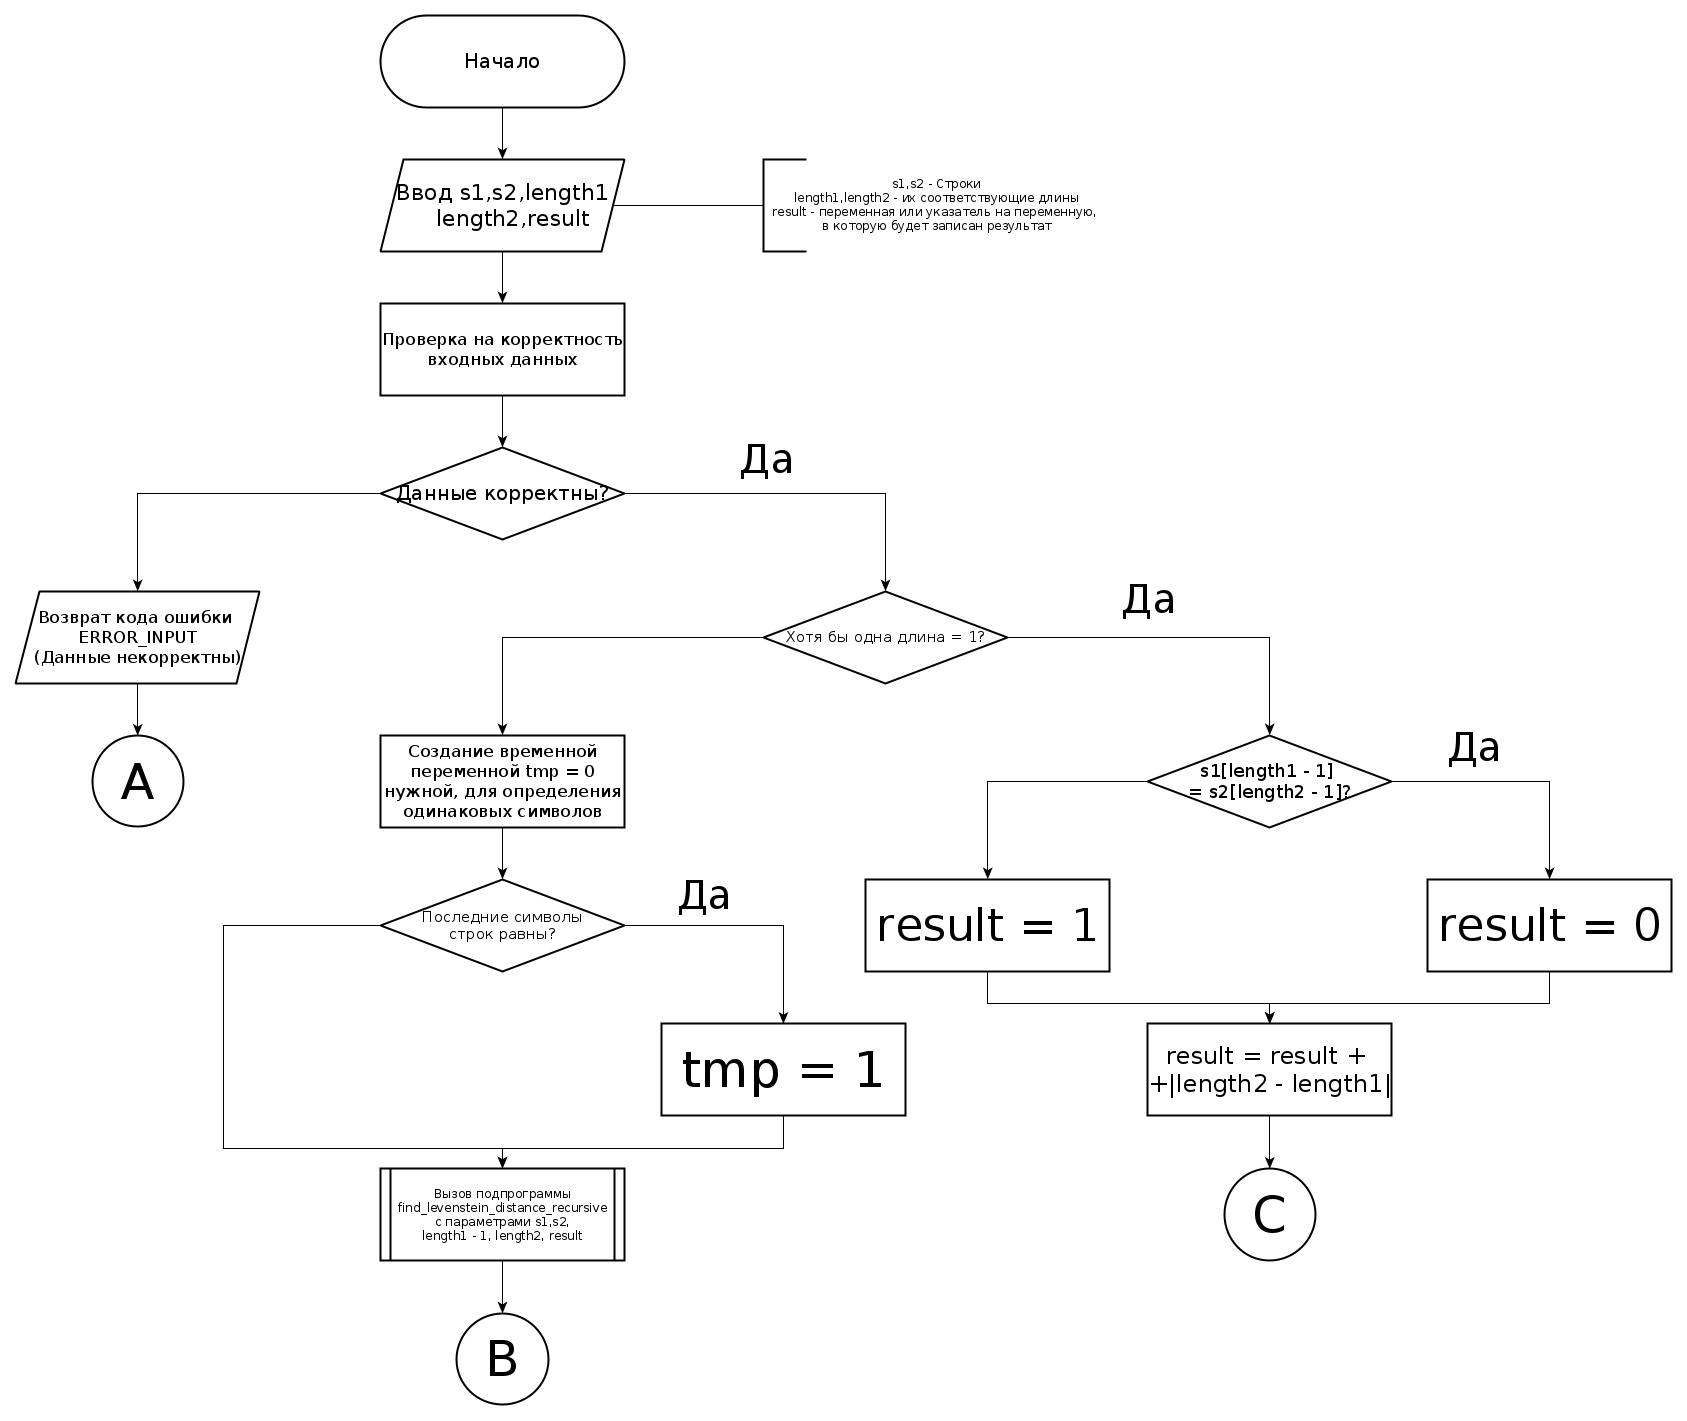
\includegraphics[scale=0.25]{recursive_levenstein.png}}
\caption{Схема рекурсивного алгоритма Левенштейна (Начало)}
\label{images:recursive_levenstein}
\end{figure}

\begin{figure}[p]
\center{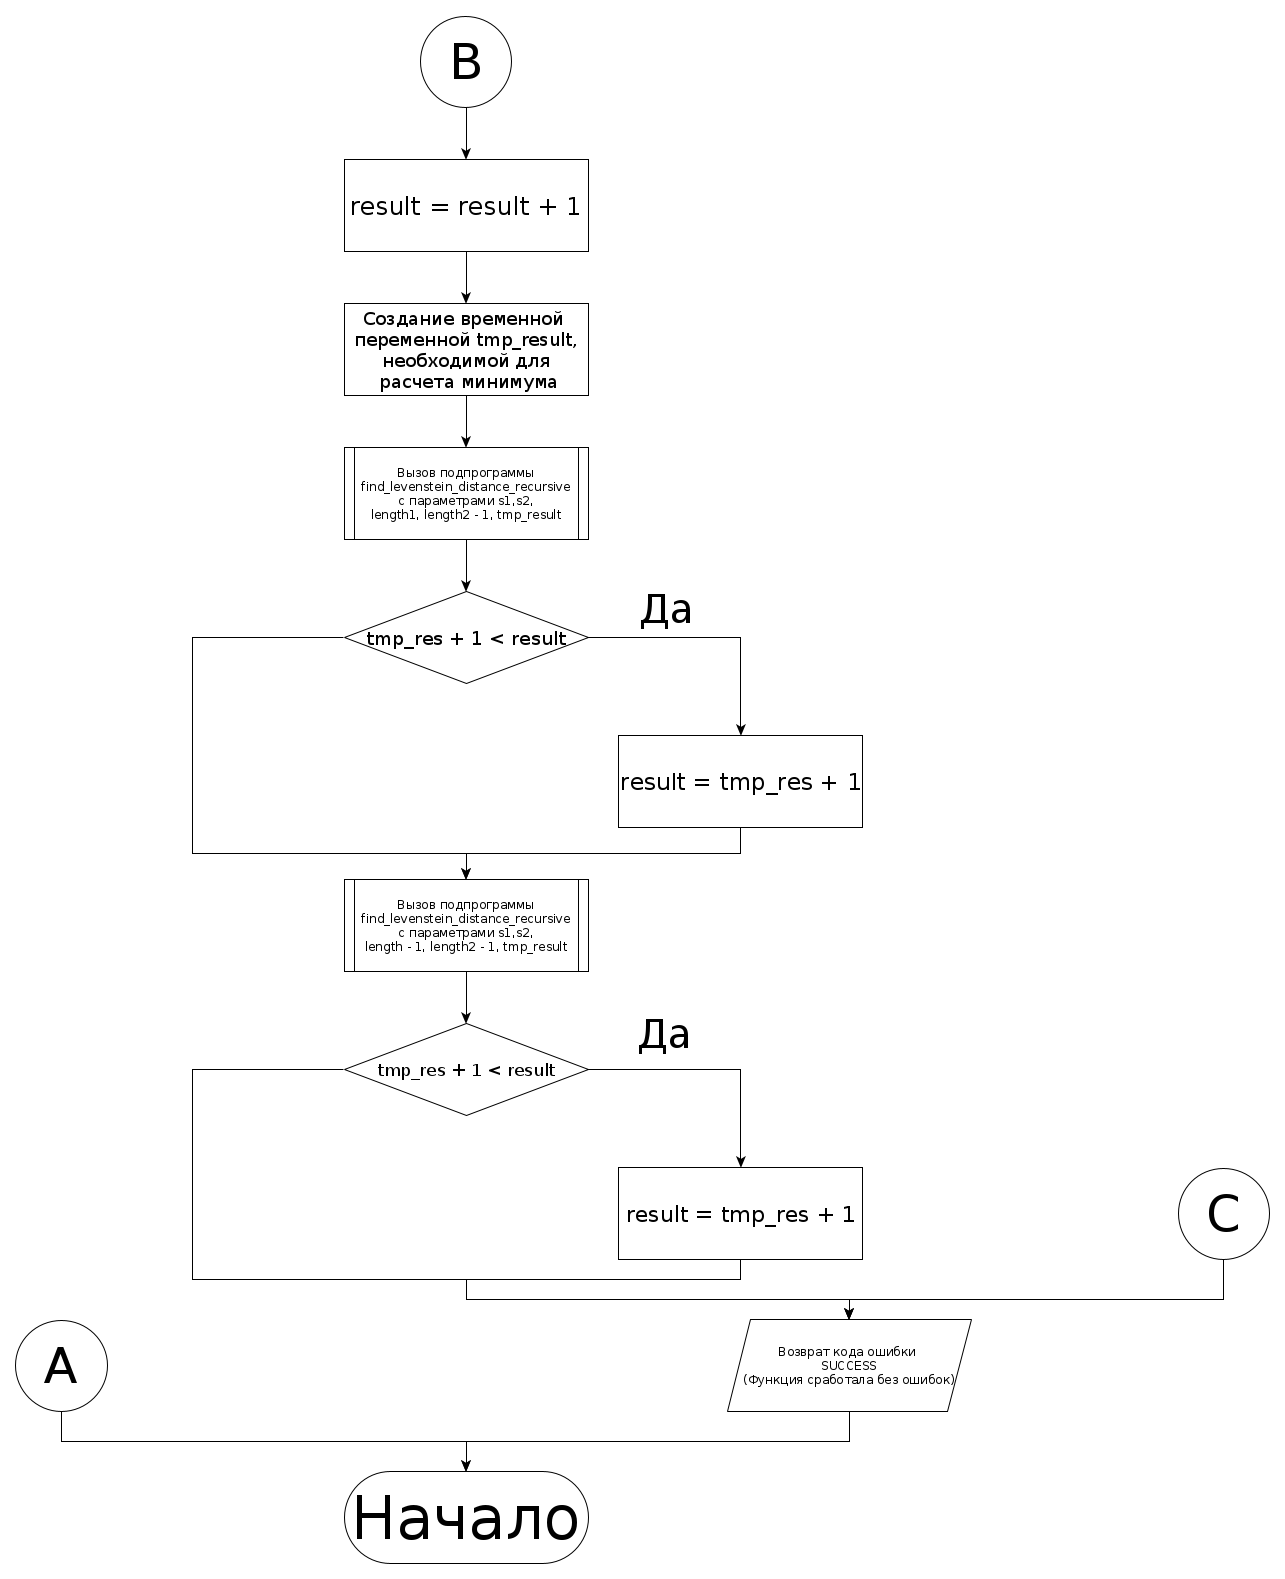
\includegraphics[scale=0.25]{recursive_levenstein2.png}}
\caption{Схема рекурсивный алгоритма Левенштейна (Конец)}
\label{images:recursive_levenstein2}
\end{figure}

\begin{figure}[p]
\center{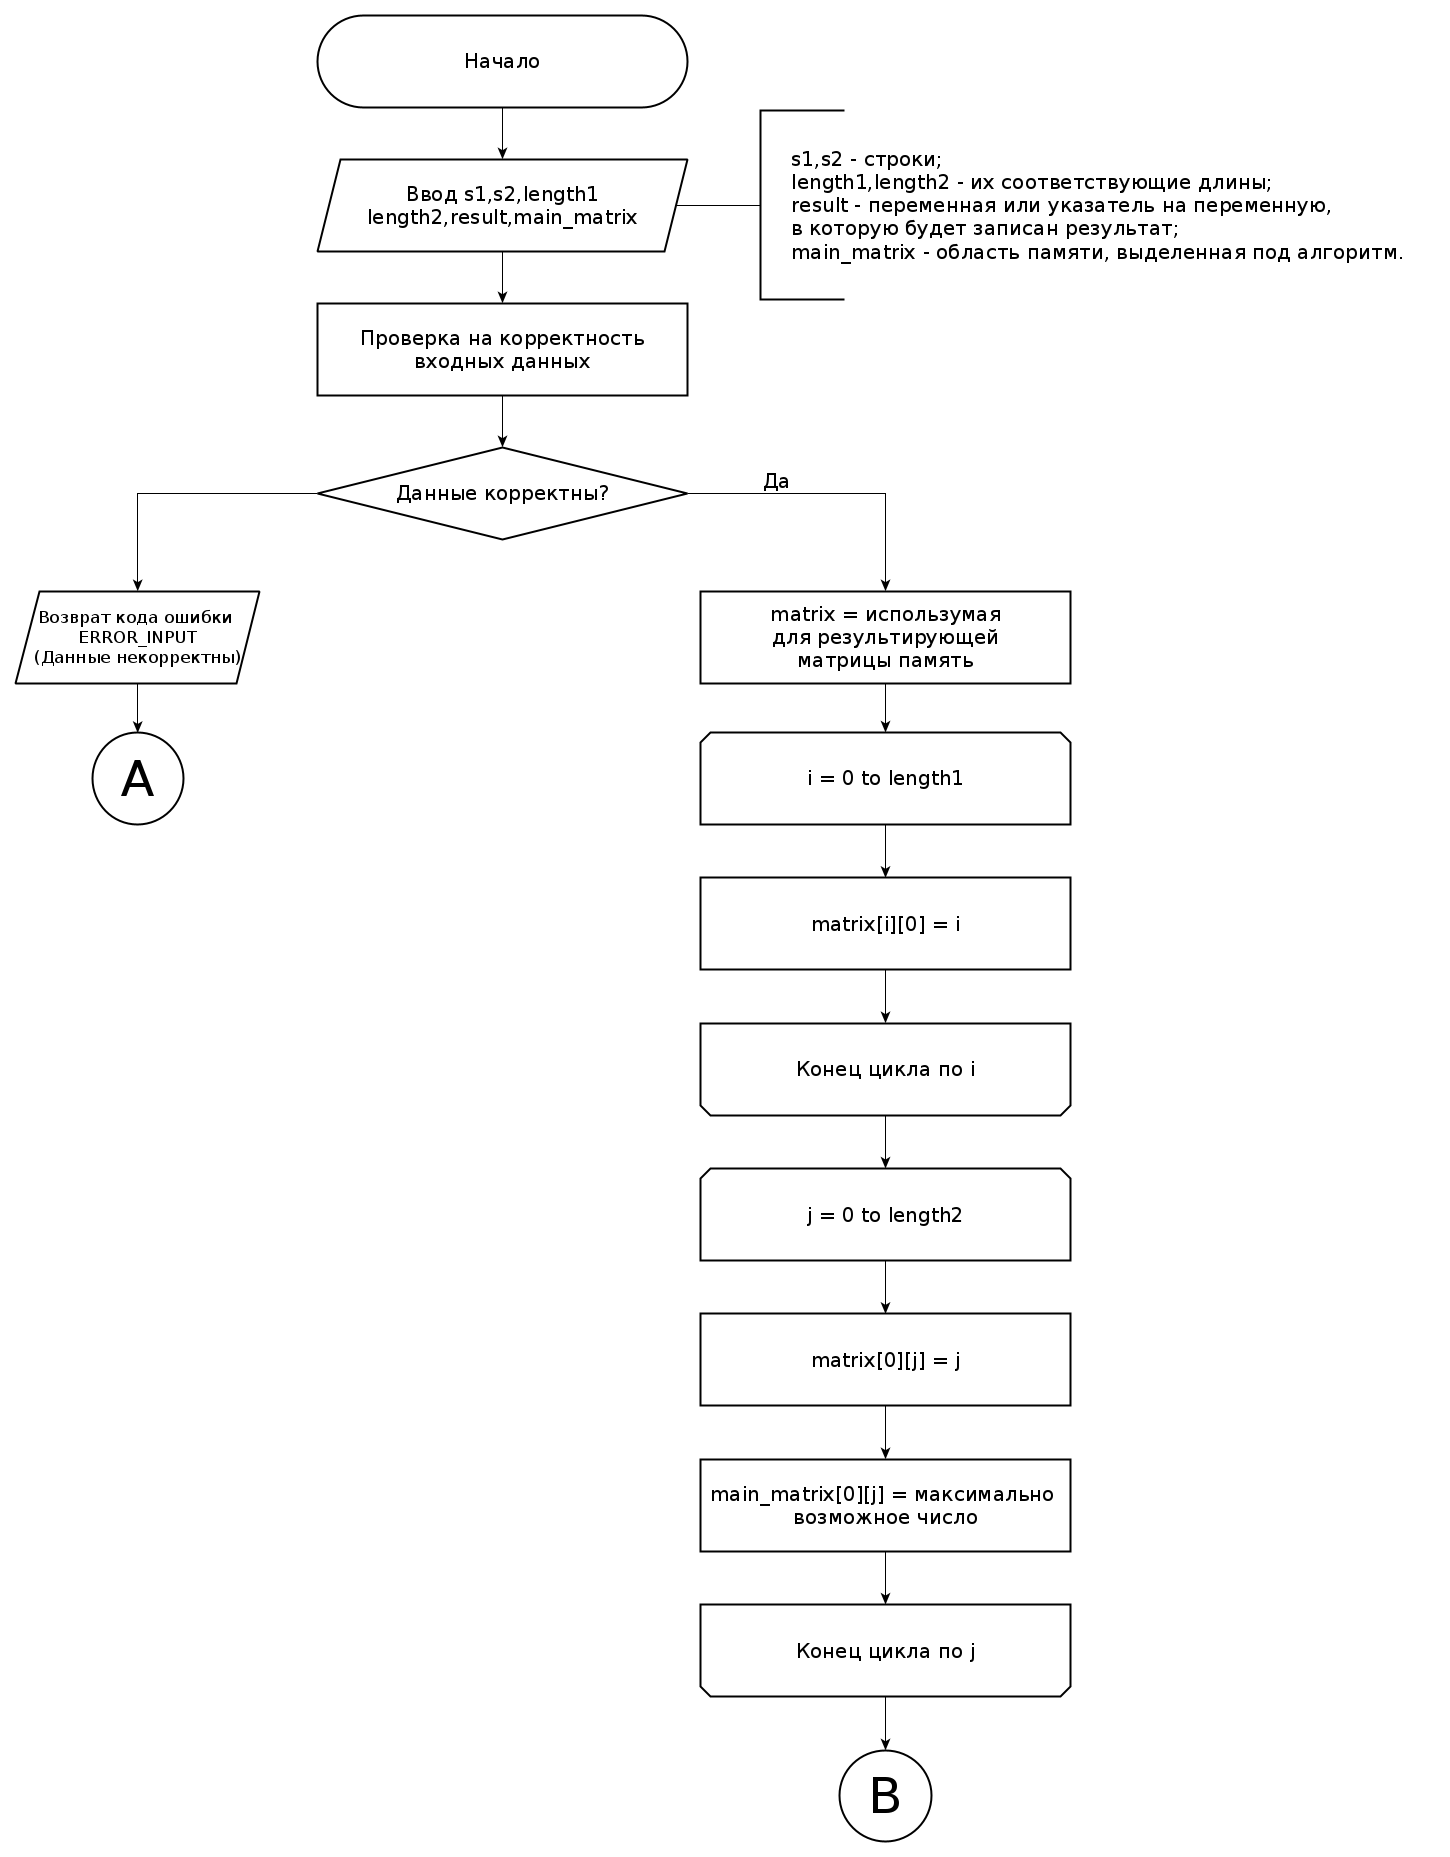
\includegraphics[scale=0.25]{damerlau.png}}
\caption{Схема стандартного алгоритма Дамерау-Левенштейна (Начало)}
\label{images:damerau_levenstein}
\end{figure}

\begin{figure}[p]
\center{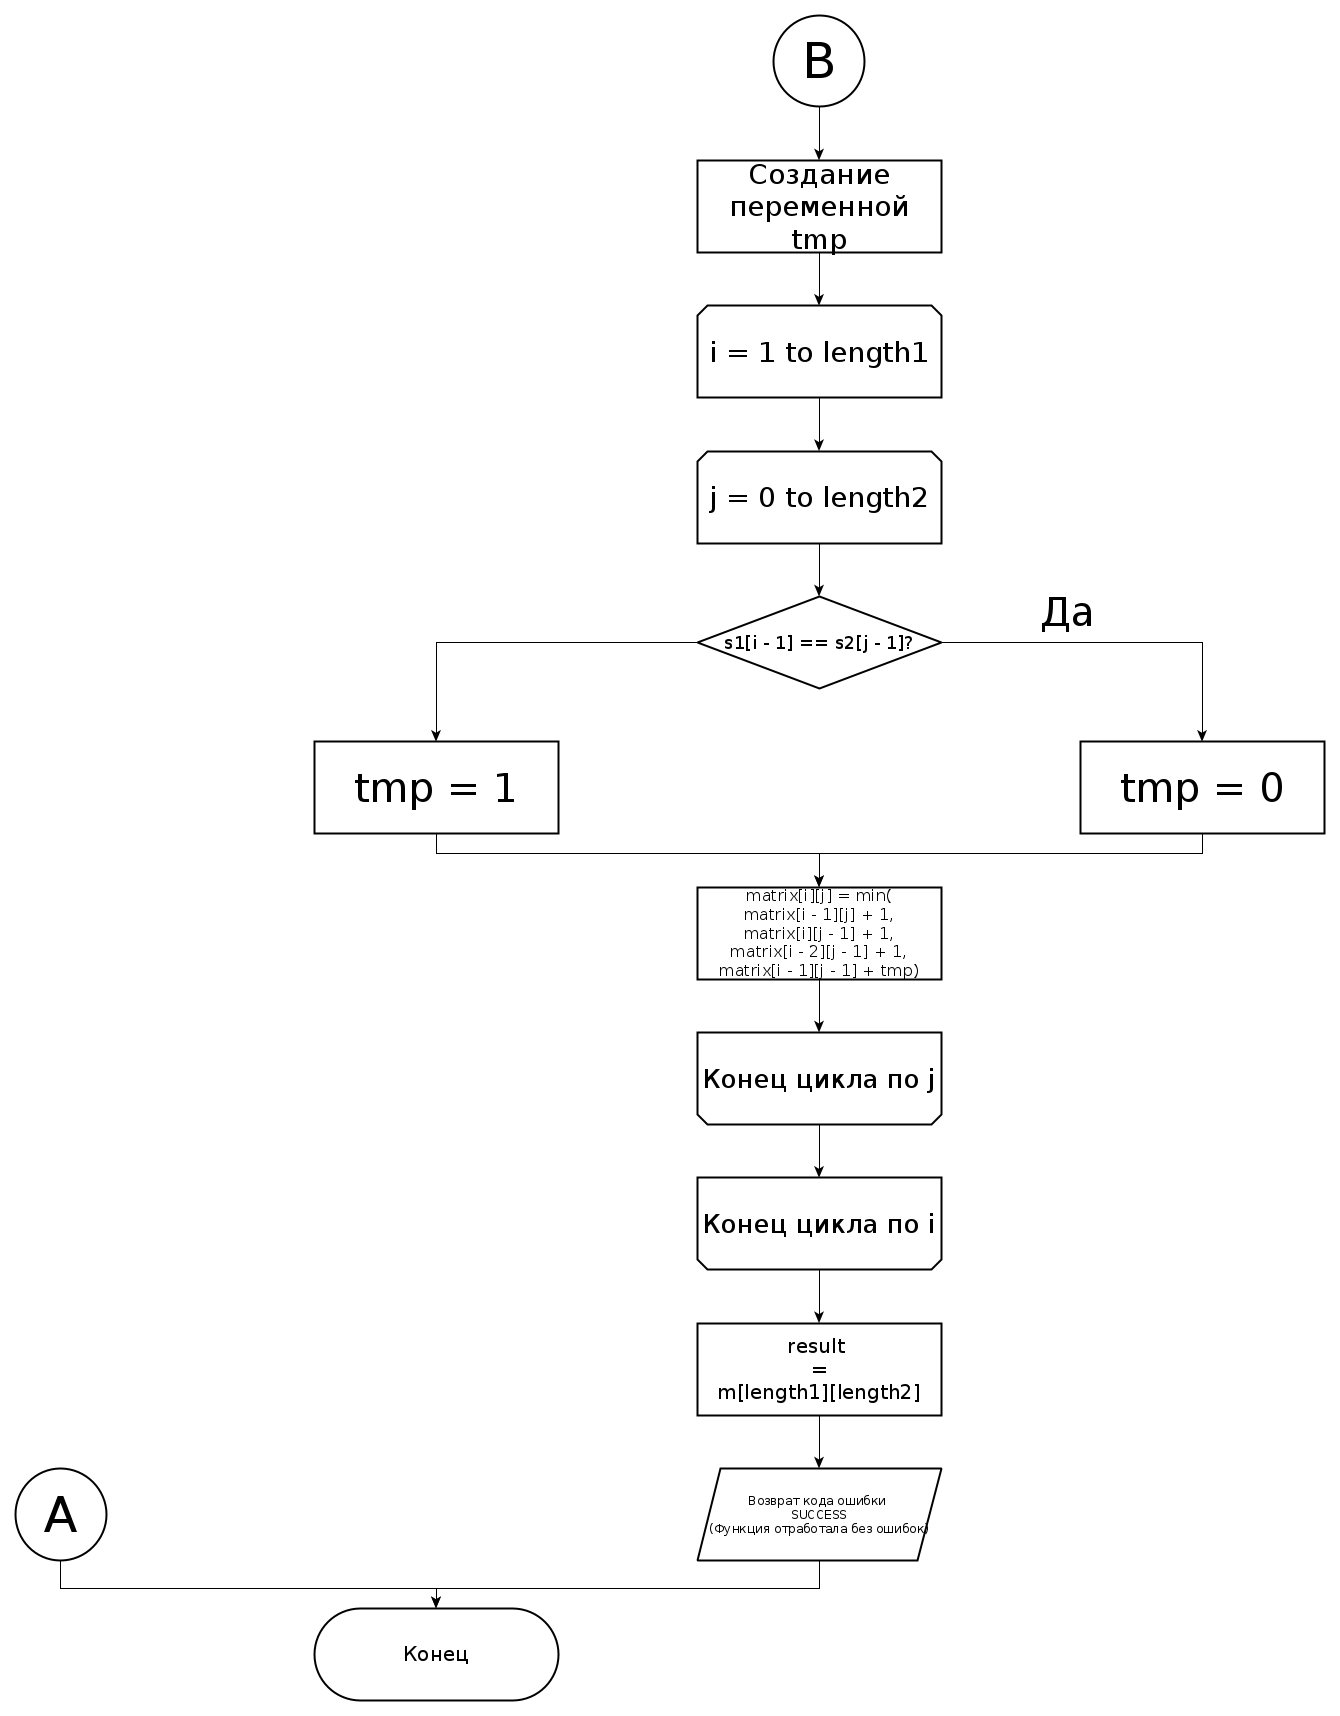
\includegraphics[scale=0.25]{damerlau2.png}}
\caption{Схема стандартного алгоритма Дамерау-Левенштейна (Конец)}
\label{images:damerau_levenstein2}
\end{figure}